\section{Annexes}

La bête à corne ci-dessous permet de mieux comprendre les fonctions principales du projet, parties prenantes et objectifs du projet. \\
\label{ann:BeteCor}
\begin{figure}[h]
   \centering
   {
       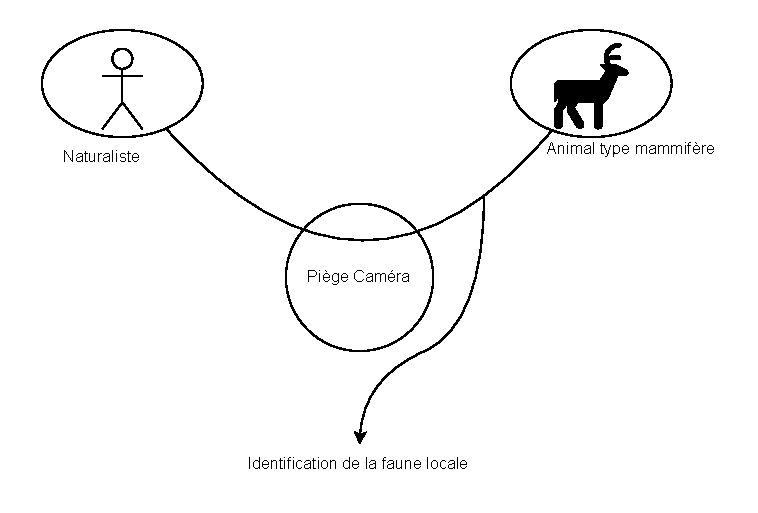
\includegraphics[width=0.7\textwidth]{images/bete_a_corne.pdf}
   }
   \caption{Bête à corne}
   \label{fig:BeteCor}
\end{figure}

\vspace{1cm}

\label{ann:DecFoncPrin}
\begin{figure}[h]
   \centering
   {
       
\includegraphics[width=1\textwidth]{images/schema_fonctionnel_principale.pdf}
   }
   \caption{Décomposition en bloc fonctionnel principale}
   \label{fig:DecFoncPrin}
\end{figure}

\label{ann:DecFoncGlo}
\begin{figure}[H]
   \centering
   {
       
\includegraphics[width=1\textwidth]{images/schema_fontionnel_global.pdf}
   }
   \caption{Décomposition en bloc fonctionnel principale et optionnelle}
   \label{fig:DecFoncGlo}
\end{figure}

\vspace{1cm}

Afin de trouver la meilleur solution technique pour chaque work package du projet, un benchmark à été mis en place dans lequel les composants ou différentes solutions sont comparées selon différents critères. \\

\label{ann:Benchmark}
\begin{figure}[H]
   \centering
   {
       
\includegraphics[width=1\textwidth]{images/schema_fontionnel_global.pdf}
   }
   \caption{Décomposition en bloc fonctionnel principale et optionnelle}
   \label{fig:DecFoncGlo}
\end{figure}

\vspace{1cm}

% \begin{table}[h!]
%     \centering
%     \scriptsize
%     \begin{tabularx}{\textwidth}{|>{\raggedright\arraybackslash}p{2cm}|>{\raggedright\arraybackslash}p{2.2cm}|>{\raggedright\arraybackslash}p{1.8cm}|>{\raggedright\arraybackslash}p{1.5cm}|>{\raggedright\arraybackslash}p{2cm}|>{\raggedright\arraybackslash}p{2cm}|>{\raggedright\arraybackslash}p{1.5cm}|>{\raggedright\arraybackslash}p{1.8cm}|>{\centering\arraybackslash}p{0.8cm}|>{\centering\arraybackslash}p{1cm}|}
%     \hline
%         \textbf{Mode} & \textbf{Principe} & \textbf{Portée typique} & \textbf{Débit indicatif} & \textbf{Avantages} & \textbf{Inconvénients} & \textbf{Coût / régulation} & \textbf{Cas d'usage} & \textbf{Énergie} & \textbf{Prix} \\
%     \hline
%         Transmission HF \\ (modulation FM) & Radio HF (3–30 MHz) \\ modulation FM & Locale à mondiale \\ selon antenne & kb/s à \\ dizaines kb/s & Très grande portée, \\ robuste & Débit limité, \\ antennes \\ encombrantes & Autorisation \\ si > 5 W & Télécom longue \\ distance, backup & 5 W & 25 € \\
%     \hline
%         LoRa & Modulation chirp \\ (LPWAN) & 0.5–15 km \\ selon environnement & 0.3 – 50 kb/s & Faible consommation, \\ grande portée & Débit limité, \\ duty-cycle & Faible coût, \\ pas d'abonnement & IoT capteurs, \\ télémétrie & 0,2 W & 30 € \\
%     \hline
%         4G (LTE) & Réseau cellulaire & Couverture \\ nationale/ \\ internationale & 1–100+ Mb/s & Haut débit, \\ mobilité, \\ bonne latence & Payant (SIM), \\ énergivore & Abonnement, \\ licences & Vidéo, cloud, \\ gros volumes & 2 W & 70 € \\
%     \hline
%         Réseau cartes \\ (filaire/sans fil) & SPI/I²C/RS485/ \\ BLE/Zigbee & $\sim$5–10 m \\ (selon solution) & Centaines kb/s \\ à plusieurs Mb/s & Simple, faible \\ latence, économique & Portée limitée, \\ dépend protocole & Faible coût & Robotique, \\ modules locaux & 0,1 W & Dépend \\ du µC \\
%     \hline
%         Wi-Fi HaLow \\ (802.11ah) & Wi-Fi sub-GHz \\ pour IoT & Jusqu'à plusieurs \\ centaines de mètres & kb/s à \\ centaines kb/s & Longue portée \\ Wi-Fi, bonne \\ pénétration & Peu répandu, \\ matériel spécifique & Puces dédiées, \\ ISM & IoT longue portée, \\ réseaux capteurs & 0,7 W & 30 € \\
%     \hline
%         ESP-NOW & Proto. Espressif \\ communication \\ directe Wi-Fi & 50–100 m (urbain), \\ 200–250 m (champ) & $\sim$1–2 Mb/s \\ (pratique <1 Mb/s) & Faible latence, \\ pas de routeur, \\ facile & Limité aux ESP, \\ pas de routage, \\ portée < LoRa & Très faible coût \\ (ESP32 < 5€) & Communication ESP \\ (robots, IoT local) & 1,5 W & 10 € \\
%     \hline
%     \end{tabularx}
%     \caption{Comparatif des modes de transmission}
% \end{table}